\documentclass[14pt, a4paper]{extarticle}

\usepackage{my_GOST}
\usepackage{hyperref}
\usepackage{listings}
\usepackage{array}
\usepackage{caption}
\hypersetup{
	pdftex,
	colorlinks = true,
	linkcolor = black,
	filecolor = magenta,
	citecolor = green,      
	urlcolor = cyan,
}

% к таблице и листингу подпись сверху, перед каждым иллюстративным материалом анонсировать
% написатьт в квадратных скобках к рекурсии комментарием что это метод и понятно почему вызываем его снова
\definecolor{mylightgray}{RGB}{240,240,240}
\definecolor{mygreen}{rgb}{0,0.6,0}
\definecolor{mygray}{rgb}{0.5,0.5,0.5}
\definecolor{mymauve}{rgb}{0.58,0,0.82}

\lstset{
	backgroundcolor=\color{mylightgray},rulecolor=\color{red},  % choose the background color; you must add \usepackage{color} or \usepackage{xcolor}; should come as last argument
	basicstyle=\fontsize{9}{11}\ttfamily,        % the size of the fonts that are used for the code
	breakatwhitespace=false,         % sets if automatic breaks should only happen at whitespace
	breaklines=true,                 % sets automatic line breaking
	captionpos=t,                    % sets the caption-position to bottom
	commentstyle=\color{mygreen},    % comment style
	extendedchars=false,              % lets you use non-ASCII characters; for 8-bits encodings only, does not work with UTF-8
	firstnumber=0,                % start line enumeration with line 1000
	frame=shadowbox,
	%rulesepcolor=\color{green},	                   % adds a frame around the code
	keepspaces=true,                 % keeps spaces in text, useful for keeping indentation of code (possibly needs columns=flexible)
	keywordstyle=\color{blue}\textbf,       % keyword style
	language=C++,                 % the language of the code
	morekeywords={*,...},            % if you want to add more keywords to the set
	numbers=left,                    % where to put the line-numbers; possible values are (none, left, right)
	numbersep=5pt,                   % how far the line-numbers are from the code
	numberstyle=\scriptsize\color{mygray}, % the style that is used for the line-numbers
	rulecolor=\color{black},         % if not set, the frame-color may be changed on line-breaks within not-black text (e.g. comments (green here))
	showspaces=false,                % show spaces everywhere adding particular underscores; it overrides 'showstringspaces'
	showstringspaces=false,          % underline spaces within strings only
	showtabs=false,                  % show tabs within strings adding particular underscores
	stepnumber=1,                    % the step between two line-numbers. If it's 1, each line will be numbered
	stringstyle=\color{mymauve},     % string literal style
	tabsize=4,	                   % sets default tabsize to 2 spaces
	title=\lstname                   % show the filename of files included with \lstinputlisting; also try caption instead of title
}
\usepackage{YATPR}

\usepackage[utf8]{inputenc}
\usepackage{amsmath}
\usepackage{float}

\begin{document}
\begin{titlepage}
	\newgeometry{pdftex, left=2cm, right=2cm, top=2.5cm, bottom=2.5cm}
	\fontsize{12pt}{12pt}\selectfont
	\noindent \begin{minipage}{0.15\textwidth}
		
\includegraphics[width=\linewidth]{pictures/b_logo.jpg}
	\end{minipage}
	\noindent\begin{minipage}{0.9\textwidth}\centering
		\textbf{Министерство науки и высшего образования Российской Федерации}\\
		\textbf{Федеральное государственное бюджетное образовательное учреждение высшего образования}\\
		\textbf{«Московский государственный технический университет имени Н.Э.~Баумана}\\
		\textbf{(национальный исследовательский университет)»}\\
		\textbf{(МГТУ им. Н.Э.~Баумана)}
	\end{minipage}
	
	\noindent\rule{18cm}{3pt}
	\newline\newline
	\noindent ФАКУЛЬТЕТ $\underline{\text{«Информатика и системы управления»}}$ \newline\newline
	\noindent КАФЕДРА $\underline{\text{«Программное обеспечение ЭВМ и информационные технологии»}}$\newline\newline\newline\newline\newline\newline\newline
	
	
	\begin{center}
		\Large\textbf{Отчет по лабораторной работе №5}\newline
	\end{center}
	
	\noindent\textbf{Название} $\underline{\text{~Моделирование работы информационного центра~~~~~~~~~}}$\newline\newline\newline
	\noindent\textbf{Дисциплина} $\underline{\text{~Моделирование~~~~~~~~}}$\newline\newline
	\noindent\textbf{Студент} $\underline{\text{Зайцева А. А.~~~~~~~~~~~~~~~~~~~~~~~~~~~~~~~~~~~~~~~~~}}$\newline\newline
	\noindent\textbf{Группа} $\underline{\text{ИУ7-72Б~~~~~~~~~~~~~~~~~~~~~~~~~~~~~~~~~~~~~~~~~~~~}}$\newline\newline
	\noindent\textbf{Оценка (баллы)} $\underline{\text{~~~~~~~~~~~~~~~~~~~~~~~~~~~~~~~~~~~~~~~~~~~~~~~~~}}$\newline\newline
	\noindent\textbf{Преподаватель}$\underline{\text{~Рудаков И. В.~~~~~~~~~~}}$\newline
	
	\begin{center}
		\vfill
		Москва~---~\the\year
		~г.
	\end{center}
 \restoregeometry
\end{titlepage}


\setcounter{page}{2}

\section{Задание}

Реализовать лабораторную работу №4 на языке GPSS.

\textbf{Задание к лабораторной работе №4.}

Промоделировать работу системы массового обслуживания, определить минимальный размер буфера памяти, при котором не будет потерянных заявок. 

Время появления заявок распределено по равномерному закону, время обработки заявки обслуживающим аппаратом -- по закону Пуассона (вариант из лабораторной работы №1). С заданной вероятностью обработанная заявка возвращается обратно в очередь на обслуживание.



\section{Теоретические сведения}

\textbf{Равномерное распределение}

Функция плотности распределения $f(x)$ случайной величины $X$, имеющей равномерное распределение на отрезке $[a, b]$ ($X \sim R(a, b)$), где $a, b \in R$, имеет следующий вид:
\begin{equation}
	f(x)=\begin{cases}
		\frac{1}{b - a}, & x \in [a, b] \\
		0, & \text{иначе}.
	\end{cases}
\end{equation}

Соответствующая функция распределения $F(x) = \int_{-\infty}^{x}f(t)dt$ принимает вид: 
\begin{equation}
	F(x)=\begin{cases}
		0, & x < a \\
		\frac{x - a}{b - a}, & x \in [a, b] \\
		1, & x > b.
	\end{cases}
\end{equation}


\subsection{Распределение Пуассона}

Дискретная случайная величина $X$ имеет закон распределения Пуассона с параметром $\lambda$ ($X \sim \Pi(\lambda)$), где $\lambda > 0$, если она принимает значения $0, 1, 2,...$ с вероятностями:

\begin{equation}
	P(X = k)= e^{-\lambda}\frac{\lambda^{k}}{k!}, \quad k \in \{0, 1, 2, ...\}
\end{equation}

Соответствующая функция распределения принимает вид:

\begin{equation}
	F(x) = P(X < x) = \sum_{k=0}^{x-1}P(X = k) = e^{-\lambda}\sum_{k=0}^{x-1}\frac{\lambda^{k}}{k!} 
\end{equation}




\section{Результаты работы программы}


Для исследования разработанная программа была выполнена при фиксированном количестве заявок $n\_tasks=1000$, фиксированных параметрах времени появления заявок (параметры $a=0$ и $b=10$ равномерного распределения), и переменных параметрах $lambda\_value$ (параметр $\lambda$ распределения Пуассона, по которому распределено время обработки заявки) и $p\_reenter$ (вероятность повторного попадания в очередь), принимающих значения 4 или 10 и 0.1 или 0.5, соотвественно. 

Для каждого набора параметров минимальный размер буфера памяти, при котором не будет потерянных заявок, равен максимальному размеру очереди THEQUEUE.

Результаты работы программы приведены в листингах~\ref{lst:1}~--~\ref{lst:4}.

%\clearpage
\begin{lstlisting}[caption = {Результат работы программы при $lambda\_value=4$ и $p\_reenter=0.1$ (максимальный размер очереди -- 11)}, label=lst:1]
START TIME           END TIME  BLOCKS  FACILITIES  STORAGES
0.000           5124.517     8        1          0
...
FACILITY         ENTRIES  UTIL.   AVE. TIME AVAIL. OWNER PEND INTER RETRY DELAY
OA                1111    0.873       4.028  1        0    0    0     0      0

QUEUE              MAX CONT. ENTRY ENTRY(0) AVE.CONT. AVE.TIME   AVE.(-0) RETRY
THEQUEUE           11    0   1111    243     2.040      9.411     12.046   0
\end{lstlisting}



\begin{lstlisting}[caption = {Результат работы программы при $lambda\_value=4$ и $p\_reenter=0.5$ (максимальный размер очереди -- 605)}, label=lst:2]
START TIME           END TIME  BLOCKS  FACILITIES  STORAGES
0.000           7983.387     8        1          0
...
FACILITY         ENTRIES  UTIL.   AVE. TIME AVAIL. OWNER PEND INTER RETRY DELAY
OA                2004    0.998       3.976  1     1237    0    0     0    604

QUEUE              MAX CONT. ENTRY ENTRY(0) AVE.CONT. AVE.TIME   AVE.(-0) RETRY
THEQUEUE          605  605   2608      3   281.952    863.089    864.083   0
\end{lstlisting}


\begin{lstlisting}[caption = {Результат работы программы при $lambda\_value=10$ и $p\_reenter=0.1$ (максимальный размер очереди -- 1239)}, label=lst:3]
START TIME           END TIME  BLOCKS  FACILITIES  STORAGES
0.000          10930.424     8        1          0
...
FACILITY         ENTRIES  UTIL.   AVE. TIME AVAIL. OWNER PEND INTER RETRY DELAY
OA                1108    0.999       9.857  1     1054    0    0     0   1237

QUEUE              MAX CONT. ENTRY ENTRY(0) AVE.CONT. AVE.TIME   AVE.(-0) RETRY
THEQUEUE         1239 1238   2345      1   631.423   2943.164   2944.420   0
\end{lstlisting}


\begin{lstlisting}[caption = {Результат работы программы при $lambda\_value=10$ и $p\_reenter=0.5$ (максимальный размер очереди -- 3034)}, label=lst:4]
START TIME           END TIME  BLOCKS  FACILITIES  STORAGES
0.000          19784.424     8        1          0
...
FACILITY         ENTRIES  UTIL.   AVE. TIME AVAIL. OWNER PEND INTER RETRY DELAY
OA                1997    1.000       9.903  1     1601    0    0     0   3033

QUEUE              MAX CONT. ENTRY ENTRY(0) AVE.CONT. AVE.TIME   AVE.(-0) RETRY
THEQUEUE         3034 3034   5030      1  1529.323   6015.262   6016.458   0
\end{lstlisting}

\clearpage
Для наглядности результаты также представлены в таблице \ref{cmp}.



\begin{table}[h!]
		\begin{center}
		\captionsetup{justification=raggedleft,singlelinecheck=off}
		\caption{\label{cmp} Таблица с результатами исследования программы}
	\begin{tabular}{|c|c|c|}
		\hline
		lambda & p   & максимальный размер очереди \\ \hline
		4      & 0.1 & 11                          \\ \hline
		4      & 0.5 & 605                         \\ \hline
		10     & 0.1 & 1239                        \\ \hline
		10     & 0.5 & 3034                        \\ \hline
	\end{tabular}
\end{center}
\end{table}

Для сравнения на рисунке \ref{pic:1} приведена таблица результатов, полученных при исследовании программы с теми же параметрами из лабораторной работы №4.



\begin{figure}[h]
	\begin{center}
		{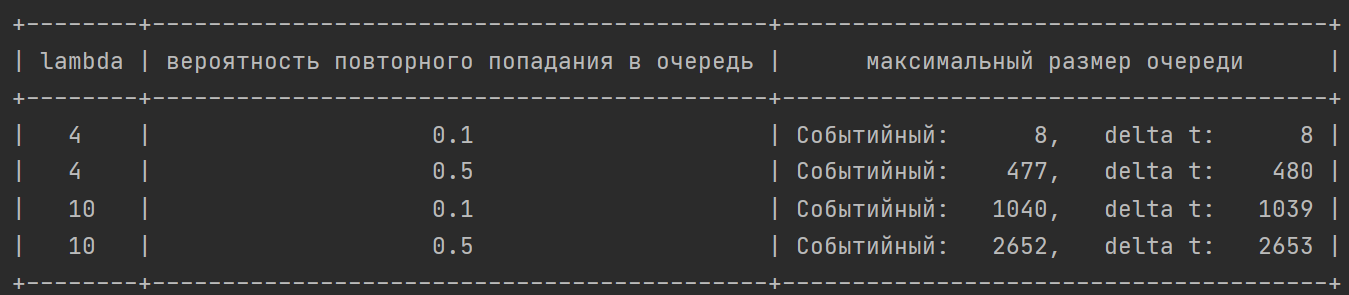
\includegraphics[scale=0.85]{pictures/res_table.png}
			\caption{Таблица с результатами исследования программы к лабораторной работе №4}
			\label{pic:1}}
	\end{center}
\end{figure}

Соответствующие результаты, полученные двумя программами, схожи (небольшие отличия вызваны случайностью генерируемых данных).

Максимальная длина очереди растет по мере роста $lambda\_value$ (так как время обработки заявки растет) и $p\_reenter$ (так как все больше заявок попадают в очередь на обслуживание повторно).

\clearpage
\section{Код программы}

В листинге \ref{lst:list1} приведен код программы. 

\begin{lstlisting}[caption = {Код программы}, label=lst:list1]
GENERATE	(UNIFORM(1,0,10))	; Время генерации заявки R(0, 10)

AddInQueue    QUEUE	TheQueue	; Вход в очередь, увеличение длины очереди
SEIZE	OA						; Захват или ожидание ОА
DEPART	TheQueue				; Выход из очереди, уменьшение длины очереди

ADVANCE	(POISSON(1,10))			; Обслуживание заявки в ОА ( время P(lambda))
RELEASE	OA						; Обслуживание заявки в ОА окончено
TRANSFER 0.1,Finish,AddInQueue	; С заданной веорятностью заявка вновь попадает в очередь

Finish	TERMINATE	1			; Окончание обслуживания заявки
START 1000						; Количество заявок
\end{lstlisting}


\end{document}